\documentclass[12pt]{article}

\usepackage{sbc-template}
\usepackage{graphicx,url}
\usepackage[utf8]{inputenc}
\usepackage[brazil]{babel}
%\usepackage[latin1]{inputenc} 
\usepackage{float}

     
\sloppy

\title{Análise Crítica de Artigo Científico sobre \\Testes de Software}

\author{Antonio Matheus Pereira de Lima\inst{1}, Fernanda Vitória Araújo Santos\inst{2},\\ João Guilherme da Silva\inst{3}, Juan do Monte Pereira\inst{4} }


\address{Análise em Desenvolvimentos de Sistemas -- Instituto Federal do Piauí (IFPI)\\
  Caixa Postal gabinete.capic@ifpi.edu.br -- 64605-5
}

\begin{document}

\maketitle

\begin{resumo}
    Este trabalho apresenta um resumo crítico do artigo científico \textit{Automated NFR testing in continuous integration environments: a multi-case study of Nordic companies}, publicado em 2023 no periódico \textit{Empirical Software Engineering}. São discutidos o problema abordado, os objetivos, a metodologia, a solução proposta, os principais resultados, as limitações e a aplicação prática da abordagem. Além disso, é apresentada uma demonstração prática baseada nos conceitos discutidos pelos autores.
\end{resumo}



\section{Introdução}

Este trabalho apresenta um resumo crítico do artigo científico \textit{Automated NFR testing in continuous integration environments: a multi-case study of Nordic companies}\nocite{yu2023automated}, de autoria de Liang Yu, Emil Alégroth, Panagiota Chatzipetrou e Tony Gorschek, publicado no periódico \textit{Empirical Software Engineering} (volume 28, artigo 144). O artigo foi aceito em 7 de junho de 2023 e disponibilizado on-line em 24 de outubro do mesmo ano. Os autores estão vinculados ao Blekinge Institute of Technology (Suécia), à Örebro University School of Business (Suécia) e à Fortiss GmbH (Alemanha).

O estudo se insere na área de Engenharia de Software, com foco em testes automatizados de Requisitos Não Funcionais (\textit{Non-Functional Requirements} -- NFRs) em ambientes de Integração Contínua (\textit{Continuous Integration} -- CI). Trata-se de um tema atual e relevante, uma vez que a automação de testes funcionais já é uma prática consolidada na indústria de software, enquanto a automação de testes de NFRs ainda representa um desafio significativo para a industria de software.

\section{Problema Estudado}

O artigo investiga como habilitar e apoiar a realizaçao de testes automatizados de Requisitos Nao Funcionais dentro de ambientes de Integração Contínua. Requisitos como desempenho, segurança, confiabilidade, escalabilidade e manutenibilidade influenciam diretamente a qualidade e o sucesso de um produto de software, além de frequentemente precisarem atender a regulamentações específicas, como o \textit{General Data Protection Regulation} (GDPR).

Apesar dessa importância, muitas organizações ainda dependem de práticas predominantemente manuais para validar NFRs, o que torna o processo menos eficiente, podendo criar gargalos nos ambientes de CI e aumentar a probabilidade de que problemas sejam identificados apenas nas fases finais do desenvolvimento. Segundo os autores, defeitos relacionados a requisitos não funcionais podem gerar retrabalho equivalente a 40\% a 50\% do esforço total de um projeto, elevando custos e comprometendo a qualidade do software entregue. Esse cenário evidencia uma lacuna prática e teórica que justifica a realização do estudo.

\section{Objetivo}

O objetivo principal do artigo é examinar como o teste automatizado de Requisitos Não Funcionais pode ser habilitado e suportado por ambientes de Integração Contínua em empresas de desenvolvimento de software. Para alcançar esse objetivo, os autores formularam quatro perguntas de pesquisa (\textit{Research Questions} -- RQs):

\begin{itemize}
    \item \textbf{RQ1:} Quais tipos de NFRs são verificados por meio de testes automatizados?
    \item \textbf{RQ2:} Quais métricas são utilizadas para testes automatizados de NFRs na prática industrial?
    \item \textbf{RQ3:} Como os ambientes de Integração Contínua contribuem para as capacidades de teste de NFRs?
    \item \textbf{RQ4:} Quais desafios estão associados aos testes automatizados de NFRs?
\end{itemize}

Essas perguntas delimitam progressivamente o escopo da investigação: partem de um levantamento descritivo (tipos de NFR e métricas empregadas) e avançam para uma análise mais aprofundada sobre a contribuição efetiva dos componentes de CI e os desafios práticos enfrentados pelas equipes.

\section{Metodologia}

A pesquisa foi conduzida por meio de um estudo de caso múltiplo, com o objetivo de investigar como empresas de desenvolvimento de software utilizam ambientes de Integração Contínua para apoiar a automação de testes de NFRs. O processo metodológico foi dividido em quatro fases:

\begin{enumerate}
    \item Planejamento, com definição dos objetivos e das questões de pesquisa;
    \item Elaboração do desenho do estudo de caso, incluindo roteiro das entrevistas, seleção dos participantes e testes-piloto;
    \item Coleta de dados por meio de entrevistas semiestruturadas;
    \item Análise temática e síntese dos dados coletados.
\end{enumerate}

A coleta de dados foi realizada por meio de 22 entrevistas semiestruturadas com profissionais da indústria de software, provindos de quatro empresas: \textit{Qvantel Sweden}, \textit{Ericsson}, \textit{Fortnox} e uma empresa anonimizada por questões de confidencialidade, identificada como \textit{Company Alpha}. Ao todo, foram analisados cinco projetos distintos (Projetos A, B, C, D e E), abrangendo domínios como finanças, telecomunicações e bem-estar social. Após a transcrição das entrevistas, os dados foram analisados por meio da técnica de análise temática, método da Engenharia de Software para identificação de padrões qualitativos.

\section{Solução Proposta}

A solução proposta pelos autores consiste em um modelo teórico-empírico que demonstra como os ambientes de Integração Contínua podem habilitar e dar suporte à automação dos testes de NFRs. O modelo mostra como os dados produzidos durante o processo de desenvolvimento são transformados em métricas capazes de avaliar continuamente a qualidade desses requisitos.

Como entradas, o modelo recebe informações produzidas durante o desenvolvimento, como alterações no código-fonte, \textit{commits} realizados no sistema de controle de versão e artefatos gerados durante o processo de \textit{build}. Como saídas, o ambiente de CI produz métricas de qualidade, relatórios de vulnerabilidades, indicadores de desempenho, tendências de qualidade ao longo do tempo e notificações automáticas que auxiliam os desenvolvedores na identificação e correção de problemas relacionados aos requisitos não funcionais.

\section{Resultados}

Os resultados, conforme apresentados na Figura \ref{fig:sintese-resultados}, indicam que os ambientes de CI possibilitam a automação de cinco tipos de NFRs: desempenho, segurança, escalabilidade, manutenibilidade e estabilidade. O requisito de desempenho foi observado em todos os projetos analisados, enquanto os requisitos de segurança estiveram presentes em quatro dos cinco projetos. Já escalabilidade, manutenibilidade e estabilidade apareceram com menor frequência, sugerindo que atributos internos ao sistema recebem menor prioridade do que atributos externos, mais visíveis ao cliente.

\begin{figure}[H]
    \centering
    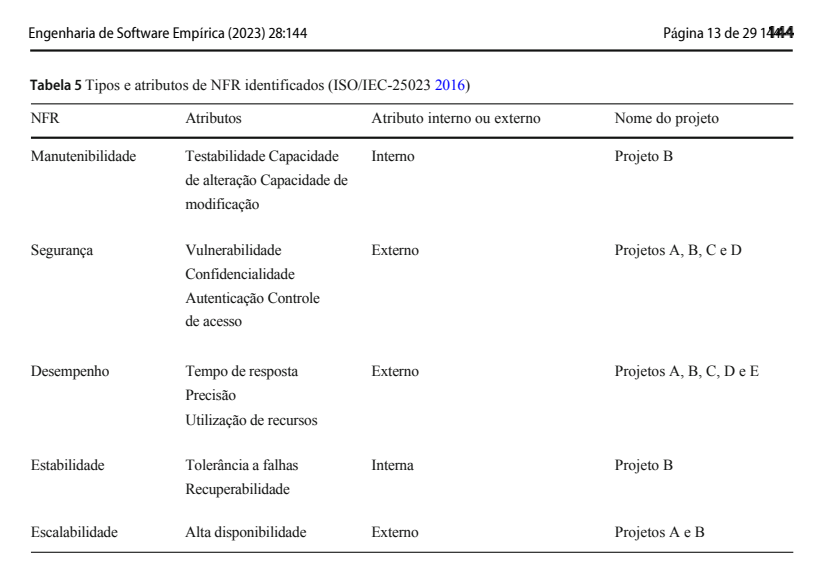
\includegraphics[width=\textwidth]{sintese-resultados.png}
    \caption{Tipos e atributos de NFR identificados. (Tabela 5 do artigo)}
    \label{fig:sintese-resultados}
    \caption*{\footnotesize Fonte: Yu et al. (2023).}
\end{figure}

Quanto às métricas, foram identificadas o Tempo Médio de Resposta (\textit{Mean Response Time} -- MRT), a Utilização do Processador (\textit{Processor Usage} -- PU) e a Precisão das Solicitações de API (\textit{Accuracy of API Requests} -- AOAR) para desempenho, além de métricas de criptografia de dados e avaliação de vulnerabilidades para segurança. Essas métricas são obtidas a partir de dados coletados pelos próprios componentes do ambiente de CI, como sistemas de controle de versão, servidores de CI, ferramentas de automação de testes, plataformas em nuvem e sistemas de rastreamento de problemas.

\begin{figure}[H]
    \centering
    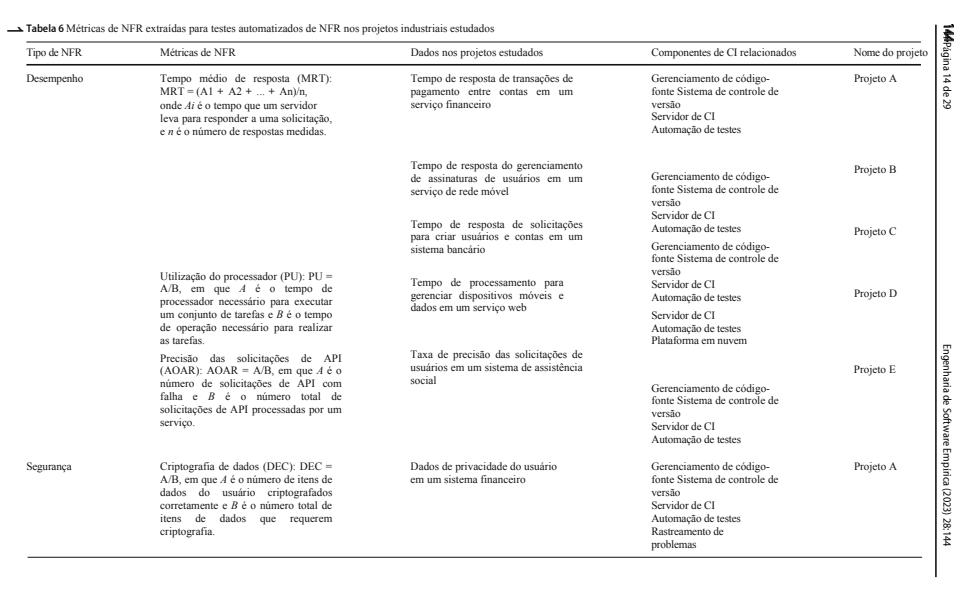
\includegraphics[width=\textwidth]{metricas-nfr.png}
    \caption{Métricas de requisitos não funcionais extraídas para testes automatizados nos projetos estudados. (Tabela 6 do artigo)}
    \label{fig:metricas-nfr}
    \caption*{\footnotesize Fonte: Yu et al. (2023).}
\end{figure}

Os autores também constataram que a utilização de ambientes de CI proporciona vantagens claras em relação aos processos tradicionais, predominantemente manuais, entre elas a detecção precoce de problemas, o monitoramento contínuo da qualidade dos NFRs e a geração automática de \textit{feedback} aos desenvolvedores, tornando o processo de desenvolvimento mais eficiente.

\section{Limitações}

Os autores reconhecem que alguns NFRs de natureza subjetiva, como a usabilidade, ainda são difíceis de automatizar e medir de forma confiável, dependendo, em grande parte, de avaliações realizadas por especialistas ou usuários. Além disso, o estudo identificou cinco desafios práticos recorrentes:

\begin{itemize}
    \item \textbf{Interdependência entre submódulos}: alterações para atender a um NFR em um módulo podem causar falhas inesperadas em outros módulos;
    \item \textbf{Dificuldade na análise de causa-raiz}, decorrente da distribuição dos NFRs entre diferentes equipes;
    \item \textbf{Baixa visibilidade} para acompanhar o ciclo de vida de um NFR, da implementação até a versão final do software;
    \item \textbf{Instabilidade dos ambientes de CI}, que pode gerar falsos positivos, especialmente em testes de desempenho;
    \item \textbf{Dificuldade em centralizar e analisar} os relatórios de teste, por falta de clareza sobre quais métricas monitorar.
\end{itemize}

Quanto às ameaças à validade, os autores discutem quatro dimensões:

\begin{itemize}
    \item \textbf{Validade interna:} possibilidade de interpretação incorreta das perguntas das entrevistas, mitigada por meio de testes-piloto.

    \item \textbf{Validade externa:} o estudo foi realizado apenas em empresas dos países nórdicos, limitando a generalização dos resultados para outros contextos.

    \item \textbf{Validade de construto:} alguns participantes poderiam deixar de relatar desafios reais, risco reduzido pela garantia de anonimato.

    \item \textbf{Validade de conclusão:} a análise temática dos dados envolve certo grau de subjetividade na interpretação dos resultados.
\end{itemize}

\section{Aplicação Prática}

A abordagem apresentada no artigo pode ser aplicada por empresas de desenvolvimento de software que já utilizam ambientes de Integração Contínua em seus processos, sendo especialmente útil para organizações que precisam monitorar continuamente requisitos como desempenho, segurança, escalabilidade e manutenibilidade. Pode ser empregada em aplicações web, sistemas corporativos, serviços em nuvem e outros projetos em que a qualidade dos requisitos não funcionais seja um fator crítico.

A técnica é aplicada durante todo o processo de desenvolvimento, integrada ao ambiente de CI, de modo que, a cada nova alteração incorporada ao código, os testes automatizados possam ser executados e as métricas de NFR atualizadas continuamente. No estudo, foram utilizadas ferramentas como JMeter, JUnit, Postman, ZAP, Anchore e SonarQube para a execução dos testes, além de Jenkins, Bitbucket, VMware e JFrog Artifactory para apoiar o processo de CI e o gerenciamento das atividades.

Com base nos resultados apresentados no artigo, a solução possui potencial para melhorar a automação dos testes de requisitos não funcionais em organizações que ja utilizam Integraço Contínua. Uma vez que ela permite o monitoramento contínuo da qualidade do software e a detecço precoce de problemas.

\section{Conclusão}

O artigo é bem estruturado e apresenta uma organização clara das informações. A divisão em introdução, fundamentação teórica, metodologia, resultados, discussão e conclusão facilita a compreensão do estudo. Além disso, os autores utilizam tabelas e figuras que contribuem para a interpretação dos resultados e para a apresentação do estudo proposto.

A metodologia adotada mostrou-se adequada aos objetivos da pesquisa. O estudo de caso múltiplo permitiu analisar práticas utilizadas em diferentes empresas de desenvolvimento de software, enquanto as entrevistas possibilitaram a obtenção de informações detalhadas sobre a utilização de ambientes de Integração Contínua para testes de requisitos não funcionais.

A técnica proposta pode ser aplicada em organizações que já utilizam ambientes de Integração Contínua e desejam aprimorar o monitoramento de requisitos não funcionais. A utilização do modelo pode contribuir para a identificação precoce de problemas e para a melhoria contínua da qualidade do software, desde que a empresa possua uma infraestrutura de CI adequada.

Como sugestão de aprimoramento, seria interessante que futuras pesquisas realizassem estudos experimentais para validar o modelo em diferentes tipos de projetos e organizações. Além disso, a inclusão de empresas de outros países e setores poderia ampliar a aplicabilidade dos resultados e fornecer evidências adicionais sobre a eficácia da abordagem proposta.


\section{Demonstração Prática}

Como forma de ilustrar, na prática, o conceito central discutido no artigo analisado, foi desenvolvido uma pequena demonstração que reproduz, de maneira simplificada, um dos exemplos apresentados pelos autores (\textit{Example 1}, Seção 4.2 do artigo): a medição automatizada de uma métrica de desempenho -- o Tempo Médio de Resposta (\textit{Mean Response Time -- MRT}) -- integrada a um \textit{pipeline} de Integração Contínua.

\subsection{Estrutura da demonstração}

A demonstração é composta por três elementos:

\begin{itemize}
    \item uma API mínima, desenvolvida em Node.js/Express, contendo uma rota simples que simula uma consulta de dados;
    \item um teste automatizado de desempenho, responsável por realizar múltiplas requisições a essa rota e calcular o MRT, utilizando a mesma fórmula apresentada na Tabela 6 do artigo (\textit{MRT = (A\textsubscript{1} + A\textsubscript{2} + ... + A\textsubscript{n}) / n});
    \item um \textit{workflow} do GitHub Actions, que executa esse teste automaticamente a cada envio de código (\textit{push}) ao repositório, reproduzindo o papel do ``servidor de CI'' descrito no modelo teórico do artigo (Figura~\ref{fig:modelo-nfr}).
\end{itemize}

\subsection{Cenário de sucesso}

No primeiro cenário, a aplicação responde dentro do limite de tempo previamente estabelecido (100 ms). O \textit{pipeline} de CI executa o teste automaticamente, calcula o MRT com base nas requisições coletadas e conclui a execução com sucesso, sinalizando que o requisito não funcional de desempenho foi atendido. A Figura~\ref{fig:demo-sucesso} apresenta a execução do \textit{workflow} nesse cenário.

\begin{figure}[H]
    \centering
    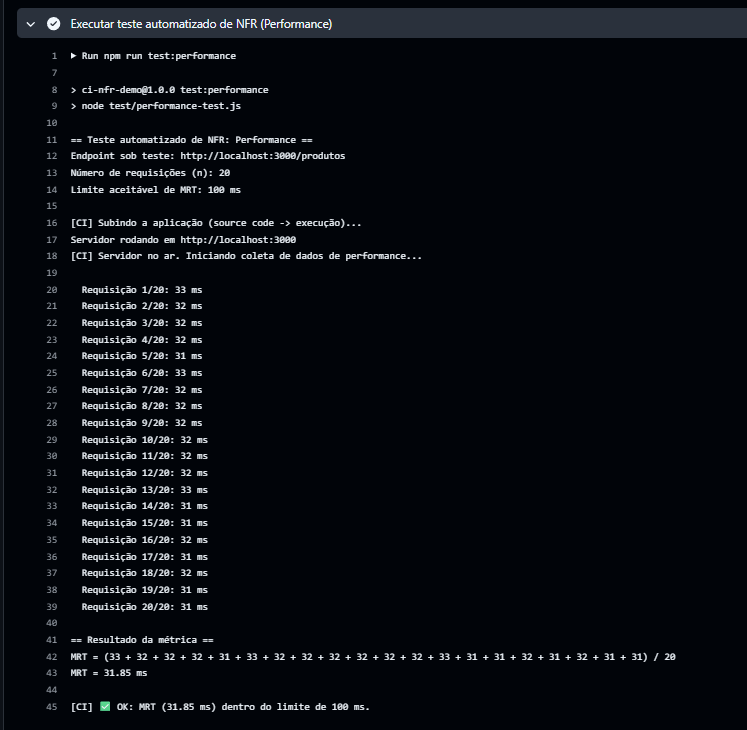
\includegraphics[width=\textwidth]{demo-sucesso.png}
    \caption{Execução do pipeline de CI com o teste de performance aprovado (MRT dentro do limite estabelecido).}
    \label{fig:demo-sucesso}
\end{figure}

\subsection{Cenário de falha}

No segundo cenário, uma latência artificial foi introduzida propositalmente no código da API, fazendo com que o MRT calculado superasse o limite de 100 ms definido no \textit{workflow}. Como consequência, o \textit{pipeline} de CI falha automaticamente, sinalizando à equipe de desenvolvimento que o requisito não funcional de desempenho não foi atendido -- exatamente o comportamento de notificação automática discutido pelos autores como um dos principais benefícios de se utilizar ambientes de CI para testes de NFRs. A Figura~\ref{fig:demo-falha} apresenta a execução do \textit{workflow} nesse cenário.

\begin{figure}[H]
    \centering
    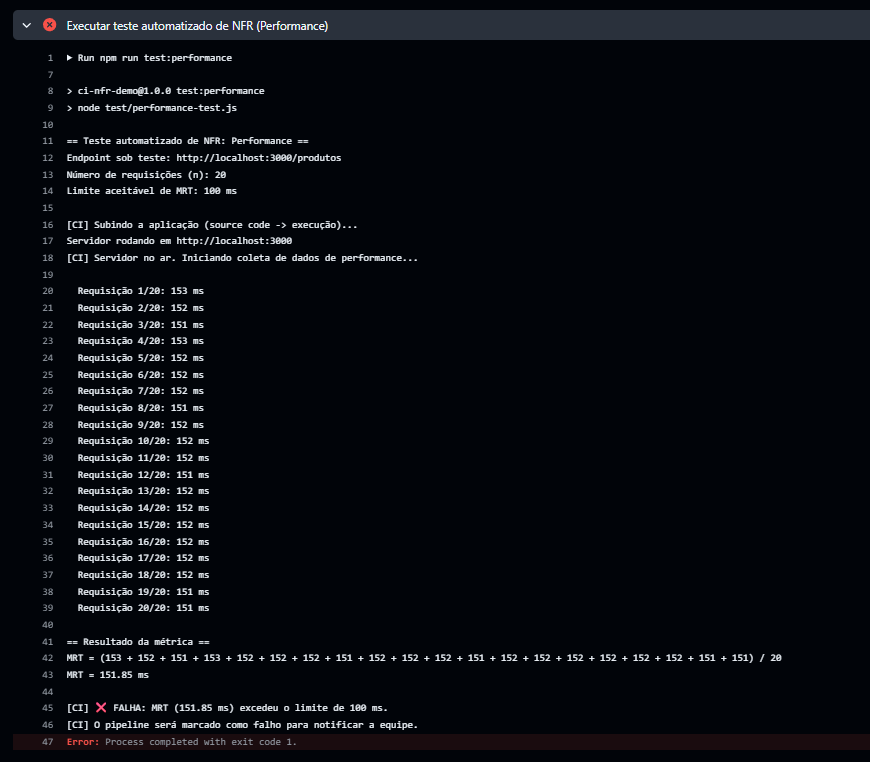
\includegraphics[width=\textwidth]{demo-falha.png}
    \caption{Execução do pipeline de CI com o teste de performance reprovado (MRT acima do limite estabelecido).}
    \label{fig:demo-falha}
\end{figure}

\subsection{Repositório da demonstração}

O código-fonte completo da demonstração, incluindo a API, o script de teste automatizado e o \textit{workflow} do GitHub Actions, está disponível no seguinte repositório:

\begin{center}
    \url{https://github.com/Fernanda135/ci-nfr-demo}
\end{center}


\bibliographystyle{sbc}
\bibliography{sbc-template}

\end{document}
